 \section{Evaluation}
 \label{sec:eval}

 {\renewcommand{\arraystretch}{1.2}
 \begin{table*}[t!]
   \centering
   \footnotesize
   \caption{Comparison of \Sys against FLASH and KAIROS. Prec.: Precision; Rec.: Recall;}
   \setlength{\tabcolsep}{0.7pt}
   \begin{tabular}{ccccccccccccc}
     \toprule
 
   \multirow{2}{*}{\textbf{Datasets}}
   & \multicolumn{4}{c }{\Norothead{ \bf \Sys}}
   & \multicolumn{4}{c }{\Norothead{ \bf FlASH}}
   & \multicolumn{4}{c }{\Norothead{ \bf KAIROS}}
   \\ \cmidrule(r{\tbspace}){2-5} \cmidrule(r{\tbspace}){6-9} \cmidrule(r{\tbspace}){10-13}
 
     & {\bf Prec.} &  {\bf Rec.} & {\bf \fscore} & {\bf TP}/ {\bf FP}/ {\bf FN}/ {\bf TN} & {\bf Prec.}  & {\bf Rec.} & {\bf \fscore} & {\bf TP}/ {\bf FP}/ {\bf FN}/ {\bf TN} & {\bf Prec.}  & {\bf Rec.} & {\bf \fscore} & {\bf TP}/ {\bf FP}/ {\bf FN}/ {\bf TN} \\
 
   \midrule
 
   E3-CADETS &  \TCP & \TCR & \TCF & \TCTP/ \TCFP/ \TCFN/ \TCTN & 0.94 & 0.99 & 0.96 & 12851/ 818/ 1/ 706,148 & 0.80 & 1.00 & 0.89 & 4/ 1/ 0/ 174 \\
   E3-TRACE &  \TTP & \TTR & \TTF & \TTTP/ \TTFP/ \TTFN/ \TTTN & 0.95 & 0.99 & 0.97 &  67382/ 3477/ 1/ 2,412,530 & - & - & - & - \\
   E3-THEIA &  \TTHP & \TTHR & \TTHF & \TTHTP/ \TTHFP/ \TTHFN/ \TTHTN & 0.92 & 0.99 & 0.95 & 25318/ 2282/ 44/ 3,503,044 & 0.91 & 1.00 & 0.95 & 10/ 1/ 0/ 216 \\  
   OpTC & \TOP & \TOR & \TOF & \TOTP/ \TOFP/ \TOFN/ \TOTN & 0.93 & 0.92 & 0.93 & 600/ 43/ 50/ 1,287,312 & 0.84 & 1.00 & 0.91 & 32/ 6/ 0/ 1210 \\
   \bottomrule
   \end{tabular}
 \label{summary:benchmarks:large}
 \end{table*}}

\Sys is developed in Python and leverages the PyTorch and Torch Geometric libraries to implement the federated graph learning framework. For developing the word2vec and vector harmonization module, we employ the Gensim library. Secure communication between clients and the utility server is ensured through Python's Cryptography module. All other functionalities of Sys are encapsulated in Python functions, designed for easy customization and deployment across different system environments.

We evaluate Sys using the open-source datasets Darpa E3 and OptC, which comprise system audit logs that simulate enterprise environments. These logs are collected from both Windows and Linux operating systems. Our evaluation experiments are conducted on a machine running Ubuntu 18.04.6 LTS, equipped with an 8-core Intel CPU and 100 GB of memory. Additionally, the machine features an NVIDIA RTX2080 GPU, utilized for operating our graph learning framework. Our evaluation aims to address the following research questions (RQs).

\begin{itemize}[leftmargin=*]
\item \textbf{RQ1.} How does \Sys compares to existing systems in terms of detection performance?
\item \textbf{RQ2.} What is the effectiveness of word2vec harmonization in a utility server setting?
\item \textbf{RQ3.} What is the resource consumption of \Sys running on a client machine?
\item \textbf{RQ4.} What is the end to end processing time of \Sys on a client machine?
\item \textbf{RQ5.} What is the effect of varying differential privacy noise on detection performance?
\item \textbf{RQ6.} Ablation study of various \Sys components.
\end{itemize}

\subsection{Datasets}
We have employed the Darpa E3 and \optc datasets for our evaluation. The E3 dataset originates from Darpa's third engagement exercise involving red and blue teams. In this exercise, the red team aimed to exploit vulnerabilities in an enterprise's services while masking their attacks with benign system activities. The logs captured from these exercises were documented under various scenario names, including Cadets, Trace, and Theia.

\optc is another open-source dataset from Darpa, encompasses a vast collection of audit logs from an enterprise environment with 1000 hosts. This dataset includes six days of benign system logs, which serve as training data for our system to understand normal behavior. Following the benign logs, there are attack logs covering three days of system activities, featuring red team tactics such as initial compromises, privilege escalations, malicious software installation, and data exfiltration.

Both datasets are accompanied by ground truth documents that help distinguish between benign and malicious events. We utilize attack labels from existing systems, such as \threatrace and FLASH, for our evaluation, cross-referencing these labels with the ground truth to ensure accuracy.

\subsection{Detectors for Comparison}

To benchmark our system, we conduct comparisons against existing state-of-the-art Provenance-based Intrusion Detection Systems (PIDS). \threatrace, a node-level system, employs graph representation learning to identify anomalous nodes within a provenance graph. In contrast, FLASH, another node-level system, surpasses \threatrace in detection efficiency and effectiveness by leveraging semantic feature vectors and an embeddings database. Given FLASH's superiority over \threatrace, our comparison focuses primarily on FLASH. Additionally, we consider KAIROS, which utilizes temporal graph networks to capture the evolution of a system's provenance graph over time. KAIROS's detection granularity is limited to specific time windows; it aggregates logs within predetermined intervals, subsequently executing anomaly detection on these collected datasets. Consequently, we extend our comparison to include \Sys versus KAIROS, focusing on their respective detection performance.

 \subsection{Detection Performance}

In this section, we discuss how \Sys compares with other systems in terms of detection performance. Initially, we outline our methodology for deploying \Sys on the DARPA E3 and \optc datasets. The E3 dataset comprises various scenarios, including Cadets, Theia, and Trace, each representing logs generated by a single host machine. To adapt \Sys for this structure, we treat each scenario as an individual host. Consequently, in our federated learning approach, we trained local \gnnshort models on each scenario individually. These local models then participated in federated averaging, a process repeated across ten rounds. Upon completing the training, we evaluated the global \gnnshort model against the attack logs from these E3 scenarios. For the \optc dataset, which is naturally divided among various hosts, we sampled three hosts for inclusion in our federated graph learning experiment. Additionally, we conducted experiments with a varying number of randomly selected hosts, the results of which are detailed in our ablation study. For conducting these evaluations, we use the same detection metrics as defined by existing node-level detectors such as \threatrace and FLASH.

Table~\ref{summary:benchmarks:large} reveals that \Sys's performance on these datasets is comparable to that of FLASH, despite the diverse log patterns and information contained within each E3 and \optc client. This underscores \Sys's capability to maintain robust detection performance amidst such heterogeneity. KAIROS's evaluation, based on a coarser time-window granularity compared to the node-level granularity of FLASH and \Sys, poses a challenge for direct comparison. Nevertheless, our results remain competitive with KAIROS.

Beyond detection performance, we also highlight \Sys's qualitative advantages, including its privacy-preserving features and distributed, scalable operation. These aspects underscore the value of \Sys in contrast to more centralized systems, emphasizing its utility in a broader range of applications.

 \subsection{Efficacy of Word2vec harmonization}

 \begin{table}[h!]
  \centering
  \small
  \setlength{\tabcolsep}{3.5pt}
    \caption{Effectiveness of word2vec vectors harmonization.}
      \begin{tabular}{ | c | c | c | c | c | c |}
        \hline
          \bf Word2vec Type & \bf Precision & \bf Recall & \bf \fscore & \bf TP & \bf FP \\
        \hline
         Local & 0.66  & 0.97 & 0.79 & 636 & 325 \\
         \hline
         Harmonized & \TOP & \TOR & \TOF & \TOTP & \TOFP \\
        \hline
      \end{tabular}
      \label{local:wordvec}
  \end{table}

 In this section, we evaluate the effectiveness of our Word2Vec vector harmonization scheme through two experiments using the \optc dataset. In the first experiment, each client utilized its locally trained Word2Vec model to encode semantic features during the training process. In the second experiment, we synchronized the individually trained models into a central Word2Vec model using the utility server architecture, as explained in Section~\ref{sec:methodology}. Then each client used this centralized model for generating semantic features. Table~\ref{local:wordvec} presents the experimental results. By employing the harmonized models, we achieved significantly better detection outcomes. This improvement is attributable to the inherent randomness of the Word2Vec algorithm, which causes different clients to produce divergent vectors for identical attributes. Such variability leads to heterogeneity in the feature vectors for the \gnnshort model, impairing the model's ability to generalize and converge effectively during the federated learning process, thereby yielding suboptimal results. However, through our novel, privacy-preserving aggregation of these semantic models, we have addressed this issue.

 \subsection{Resource Consumption of \Sys}

 In this section, we analyze the resource consumption of our system. To accomplish this, we processed batches of audit events of varying sizes using our system to model the resource utilization on a client machine comprehensively. The results, as depicted in Figure~\ref{fig:resource}, indicate that the resource consumption of \Sys is moderate. Specifically, \Sys is capable of processing up to 100,000 audit events simultaneously while consuming less than 900 MB of memory and utilizing less than 20\% of CPU resources. This suggests that \Sys does not significantly burden the client machine, particularly given that client machines typically experience low event throughput. Consequently, our system requires execution only a few times per day to process newly accumulated events, implying that resource consumption is not continuous but occurs at specific intervals. Furthermore, our analysis of the host data in the \optc dataset reveals that, on average, each client generates approximately 100,000 audit log events within a three-hour period.

 \begin{figure}[t!]
  \centering
  \subfloat[CPU Utilization.]{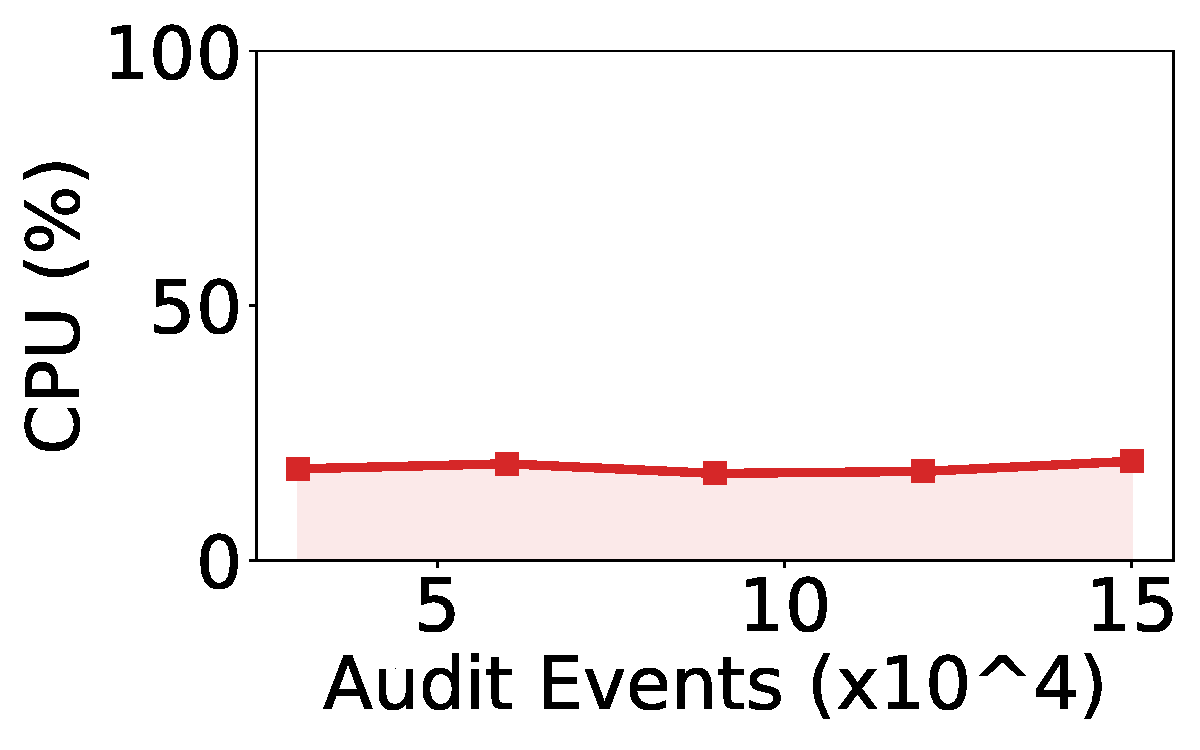
\includegraphics[width=0.24\textwidth]{fig/cpu.pdf}\label{cpu}}
  \hfill
  \subfloat[RAM Utilization]{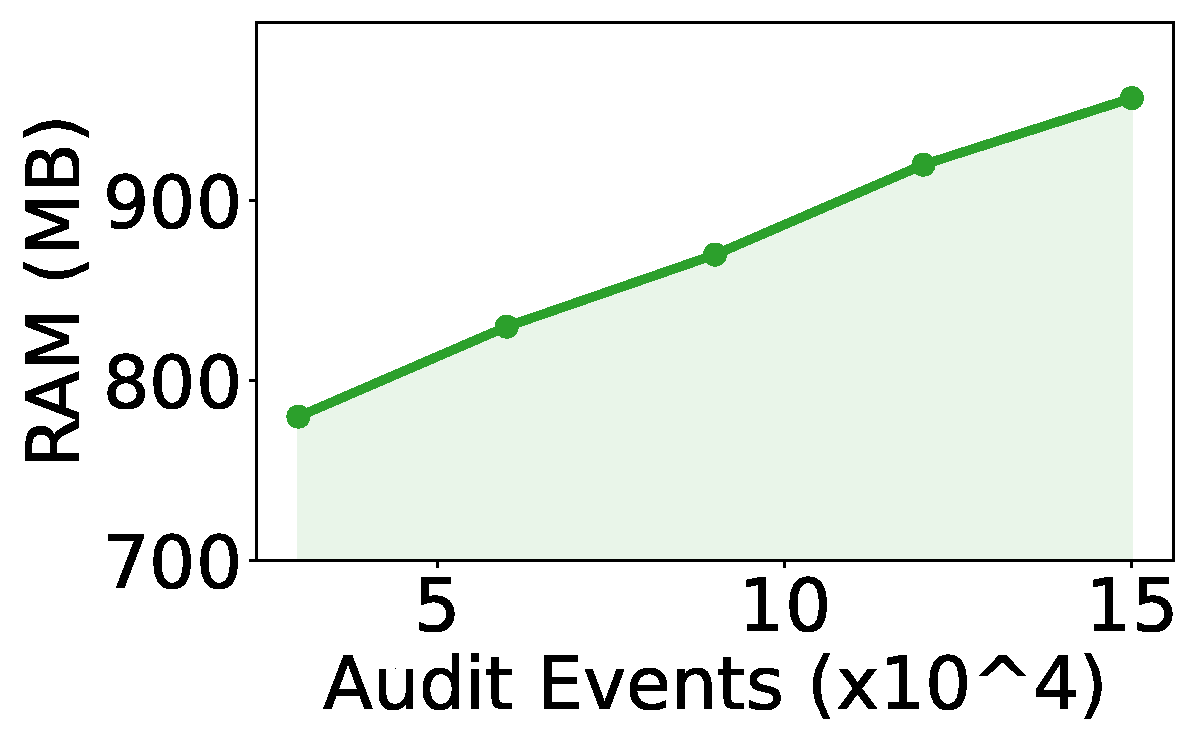
\includegraphics[width=0.24\textwidth]{fig/ram.pdf}\label{ram}}
  \hfill
  \caption{Resource Consumption of \Sys.}
  \label{fig:resource}
  \vspace{-2ex}
\end{figure}

 \subsection{Processing Time Analysis of \Sys}

 In this section, we evaluate the processing time required by our system, \Sys, to handle audit events on client machines. We experiment with batches of audit events of various sizes, conducting end-to-end inference with \Sys to measure the time taken to process these events on a client machine. The results, illustrated in Figure~\ref{sizevstime}, demonstrate that \Sys processes events with notable efficiency. For example, it requires approximately 23 seconds to process a batch of 100,000 events. Given our previous analysis of host logs in the \optc dataset, which indicated that each host generates an average of 100,000 events in three hours, \Sys can process 24 hours worth of log data on a client in merely 3 minutes. This level of efficiency ensures that our system is highly effective, preventing any potential log congestion.

 \begin{figure}[t!]
  \centering
  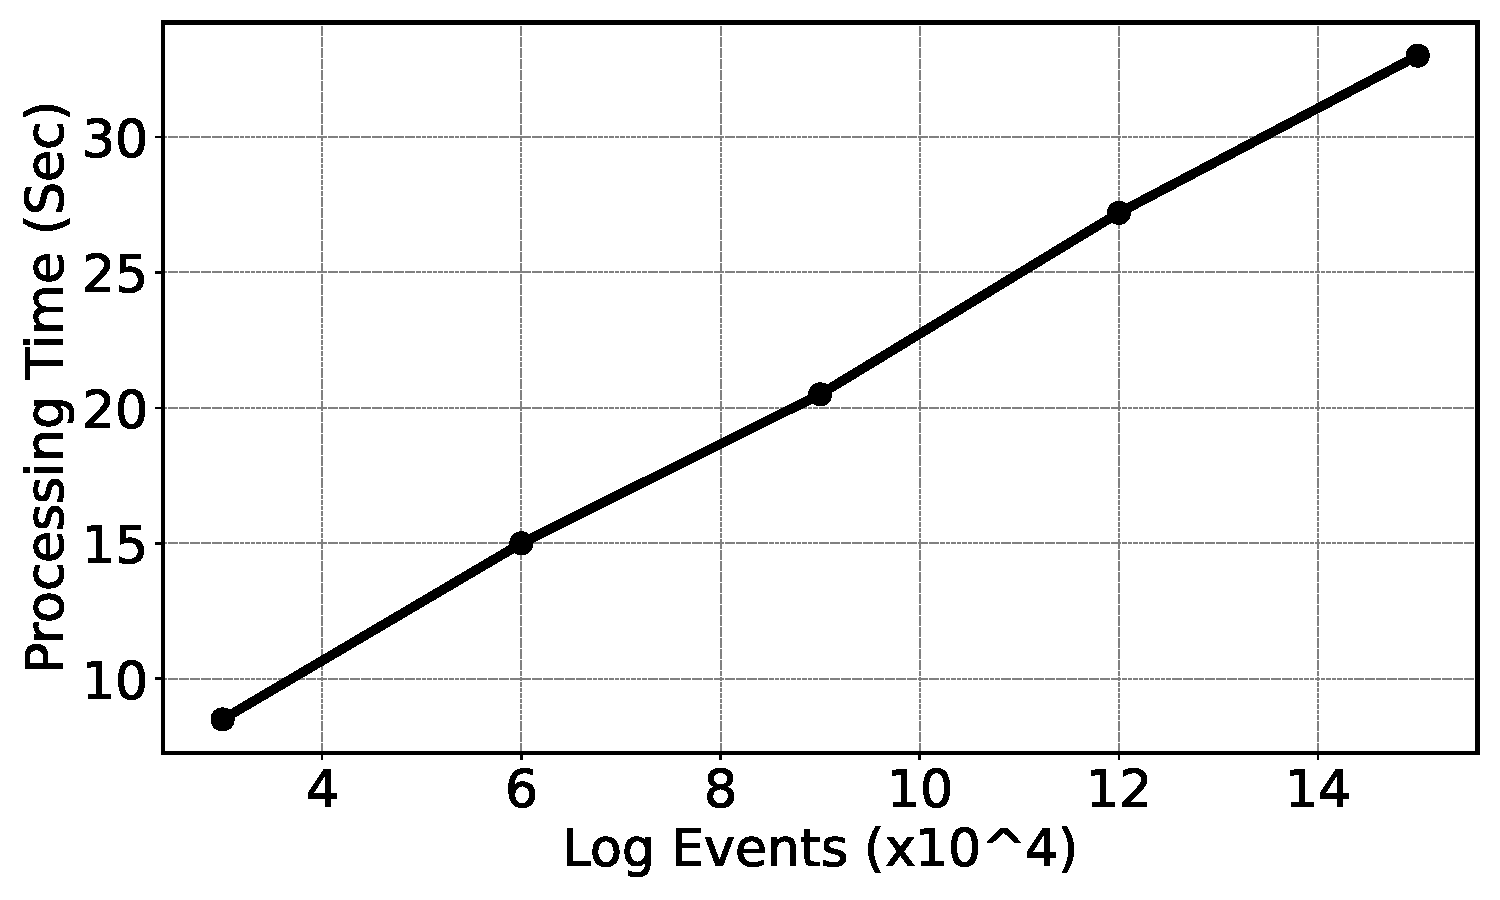
\includegraphics[width=0.48\textwidth]{fig/sizevstime.pdf}
  \caption{Processing Time for various Audit Event Sizes}
  \label{sizevstime}
  \vspace{-2ex}
\end{figure}

 \subsection{Effect of Local Differential Privacy}

 \begin{figure}[t!]
  \centering
  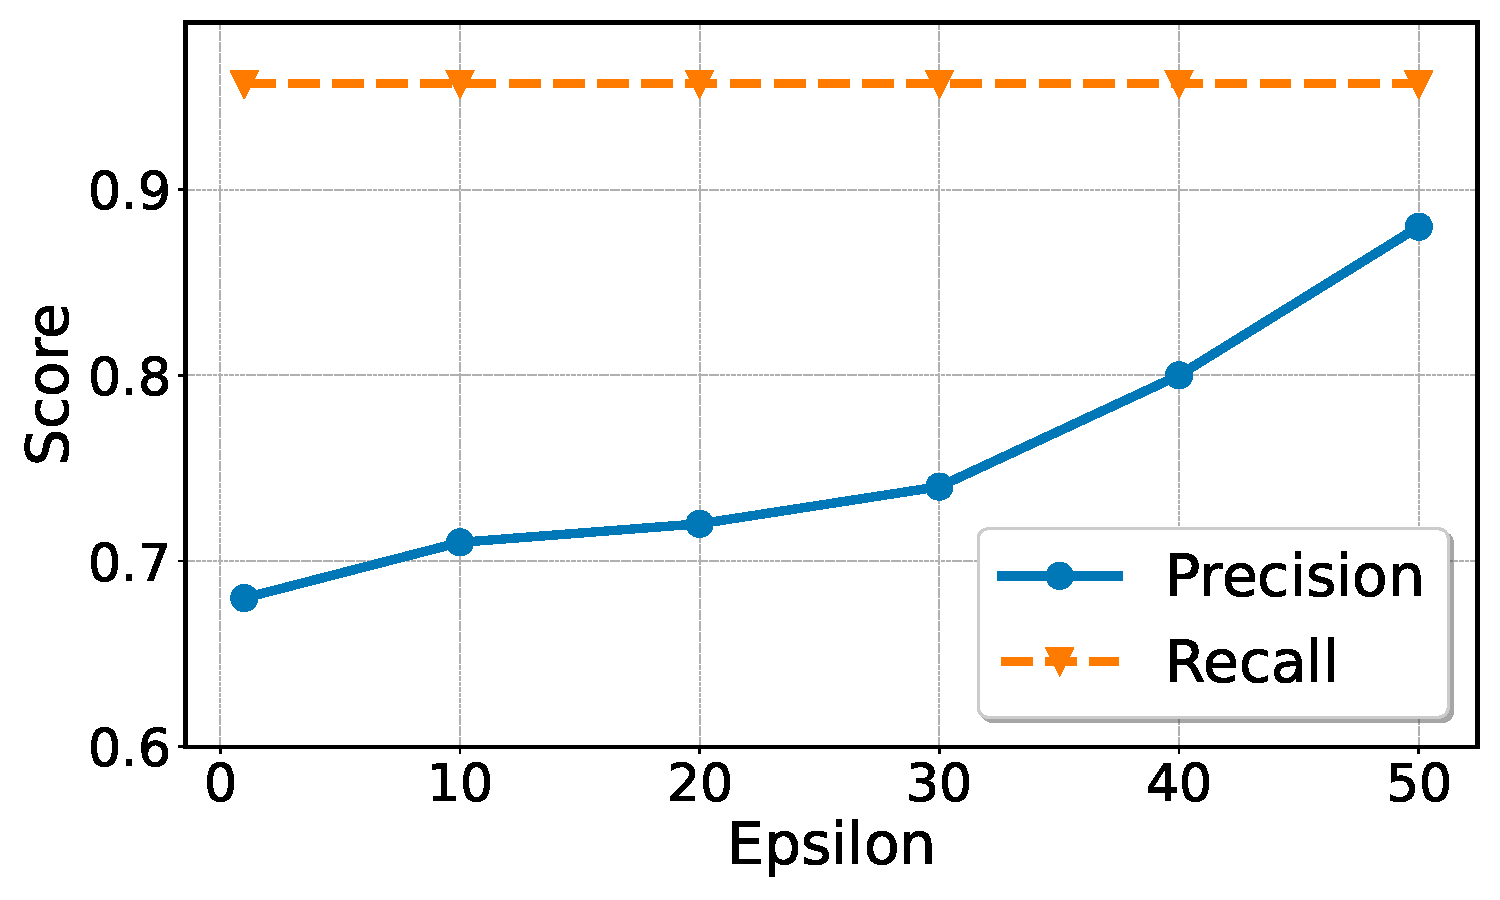
\includegraphics[width=0.48\textwidth]{fig/epsvsscore.pdf}
  \caption{Effect of Epsilon ($\epsilon$) on Detection Performance.}
  \label{epsvsscore}
  \vspace{-2ex}
\end{figure}

 In this section, we examine the impact of differential privacy noise levels on the detection performance of \Sys. Differential privacy introduces a parameter, $\epsilon$, which dictates the intensity of Gaussian noise added to the local \gnnshort model updates prior to their aggregation at the central server for federated averaging, as detailed in Section~\ref{sec:methodology}. By adjusting $\epsilon$ during the training phase, we assess the detection capabilities of the globally trained model across various $\epsilon$ settings. Figure~\ref{epsvsscore} illustrates the relationship between $\epsilon$ and detection performance. It is important to note that lower $\epsilon$ values correspond to higher noise levels in model updates, thereby strengthening privacy at the expense of model utility. Conversely, increasing $\epsilon$ reduces noise strength, improving detection performance. The optimal $\epsilon$ value is contingent upon the specific requirements and context of the organization employing \Sys, balancing between privacy protection and model utility.


 \subsection{Ablation Study}

 In this section, we analyze the impact of key parameters within \Sys. Specifically, we focus on two principal parameters: $N$, representing the number of client machines participating in Federated Graph Learning, and $R$, denoting the number of rounds the federated averaging process is executed. The effect of these parameters is discussed below: \\

\PP{Hosts vs Detection Performance} We utilized the \optc dataset for this experiment, randomly selecting a variable number of hosts to participate in training our model through federated learning. The trained global model was then applied to perform threat detection, with the outcomes documented accordingly. Figure~\ref{scoresvshosts} presents these results, illustrating that performance improvement is observed up to a certain number of hosts. This plateau is attributed to the \optc dataset's finite set of benign patterns that can be learned. Beyond this threshold, additional hosts do not contribute new information beneficial to the model, thus halting further performance gains and increasing the risk of overfitting. To mitigate this, client machines can monitor and report the loss of the global model on their local datasets, providing a metric for the server to determine the optimal point to cease the learning process. \\

\begin{figure}[t!]
  \centering
  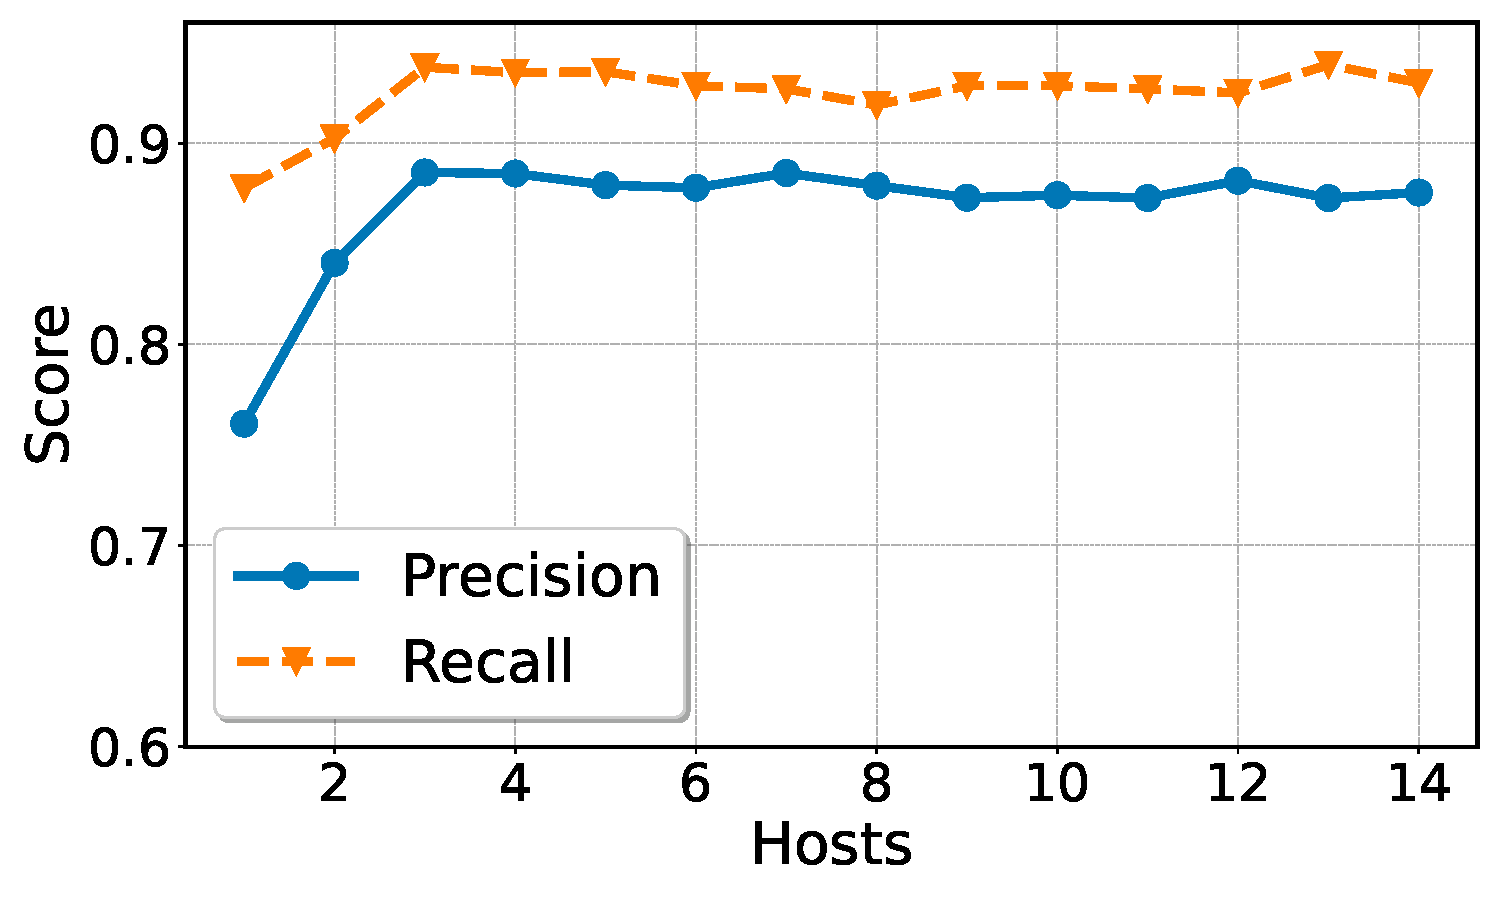
\includegraphics[width=0.48\textwidth]{fig/scoresvshosts.pdf}
  \caption{Effect of number of hosts vs detection metrics.}
  \label{scoresvshosts}
  \vspace{-2ex}
\end{figure}

\PP{Effect of Federated Averaging Rounds} We employed the Darpa E3 dataset to examine the impact of federated averaging rounds on detection performance. Our methodology involved training the model over a range of federated averaging rounds and subsequently evaluating the model's detection capabilities. The outcomes are depicted in Figure~\ref{roundsvsscore}, which shows that detection performance improves up to a certain number of rounds before declining due to overfitting. Notably, this inflection point is also characterized by a minimal decrease in training loss, suggesting that the model has reached its learning capacity. This observation proves to be a valuable metric for determining the optimal moment to stop training, thereby preventing overfitting and ensuring optimal model performance.

\begin{figure}[t!]
  \centering
  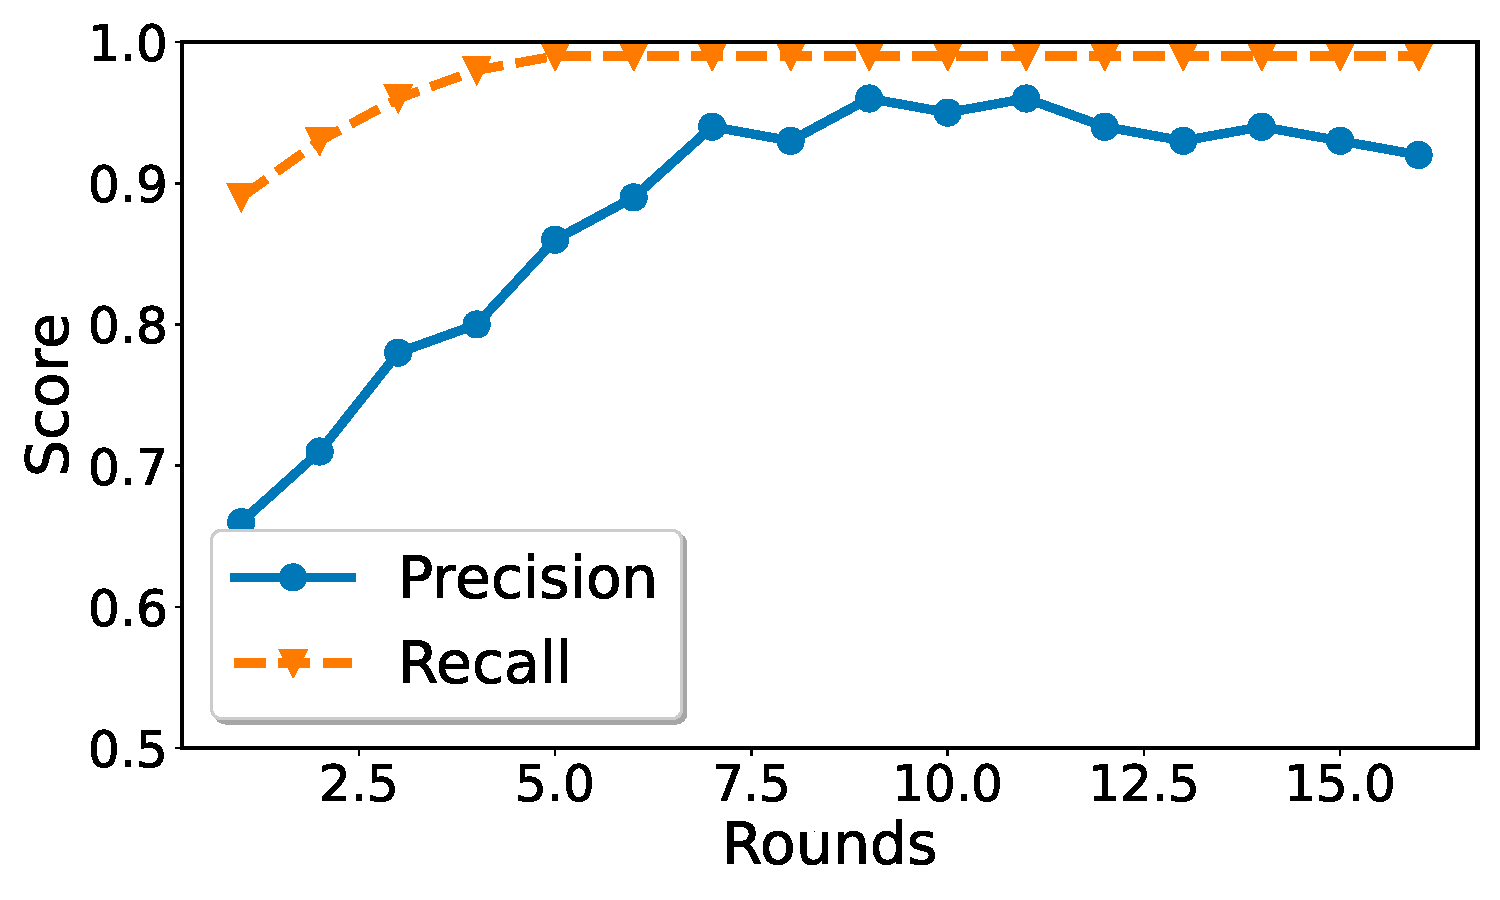
\includegraphics[width=0.48\textwidth]{fig/roundsvsscore.pdf}
  \caption{Federated Averaging Rounds vs Detection Performance.}
  \label{roundsvsscore}
  \vspace{-2ex}
\end{figure}

% \begin{figure}[t!]
%   \centering
%   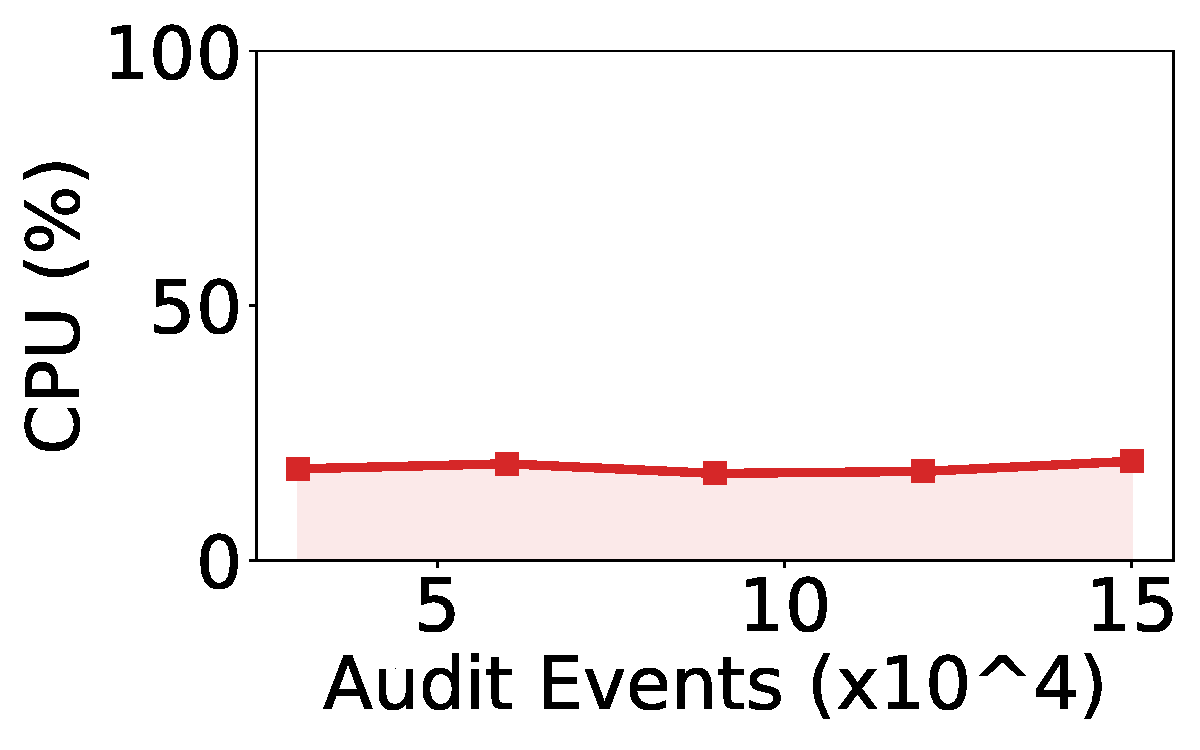
\includegraphics[width=0.40\textwidth]{fig/cpu.pdf}
%   \caption{CPU Usage}
%   \label{cpu}
%   \vspace{-2ex}
% \end{figure}

% \begin{figure}[t!]
%   \centering
%   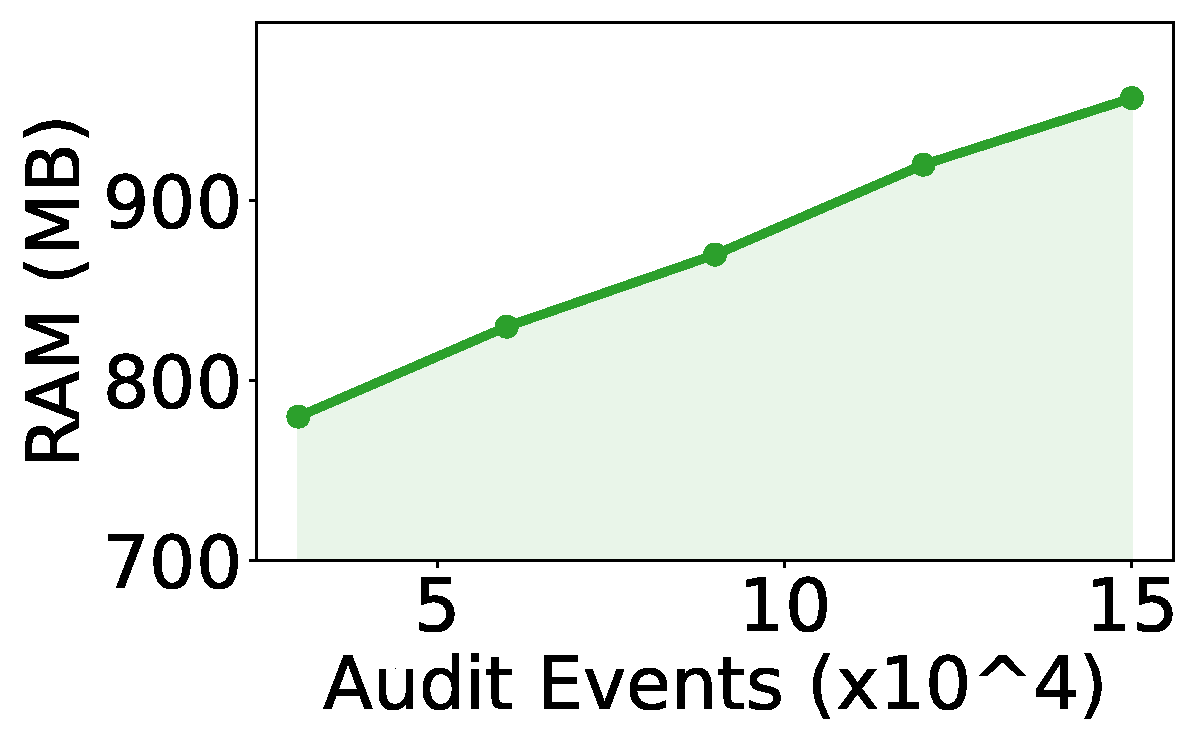
\includegraphics[width=0.40\textwidth]{fig/ram.pdf}
%   \caption{RAM usage}
%   \label{ram}
%   \vspace{-2ex}
% \end{figure}